\chapter{Verifica e validazione}
\label{cap:verifica-validazione}

Il seguente capitolo ha lo scopo di mostrare le tecniche di verifica e validazione del progetto, secondo le linee guida apprese durante il corso di Ingegneria del Software. \\
Verificare un prodotto ha l'obiettivo di controllare se l'introduzione di nuovi elementi nel codice ha generato dei problemi e se rispetta i requisiti designati. 
\\La validazione serve ad approvare il progetto qualora soddisfi tutti i requisiti imposti.

\section{Processo di Verifica}
Il processo di verifica è stato attuato durante tutto lo sviluppo del progetto per verificare le nuove funzionalità e comportamenti introdotti.\\
L'approccio all'introduzione di nuovi elementi con le relative funzioni è stato costantemente controllato da \textit{Roberto Martina}, responsabile di stage. Infatti  la tecnica più efficiente per lo sviluppo del codice è codificare una delle parti di webapp, verificare che il codice appena introdotto funzioni correttamente nel suo insieme e soltanto dopo collegarlo alle altri parti di codice già sviluppate.\\
Quindi, non si procede per codificare il "tutto" perché i requisiti potrebbero essere non soddisfatti e c'è il rischio di perdere l'obiettivo durante lo sviluppo; ma è rigoroso procedere per passi e per ognuno verificarne la correttezza.

\subsection{Debbuging}
Una delle tecniche per verificare il giusto funzionamento dell'applicazione è il \textit{\textbf{Debugging}}. Effettuando il debug significa controllare a \textit{run-time} come si comporta l'applicazione durante l'interazione con l'utente. Dopo aver introdotto una nuova funzione per l'applicazione si può effettuare il debug per verificare che la funzione introdotta funzioni nel corretto modo e non vada a creare problemi con gli altri elementi già presenti. \\
Lo strumento di \textit{debug} utilizzato per verificare il progetto è quello messo a disposizione da \textbf{IDE Eclipse}. \textit{Eclipse} mette a disposizione sia il \textit{debug} del codice, ma anche il \textit{debug} per il server su cui viene eseguita la webapp.
Inoltre, una feature di Eclipse, introduce la possibilità di inserire dei \textit{breakpoint} che permettono di verificare il codice linea per linea.\\ Inserendo un \textit{breakpoint} su una riga, 'applicazione si fermerà su quel \textit{breakpoint} durante la sua esecuzione e il programmatore con i tasti F,F10,F11,F12 potrà proseguire per ogni riga in modo da individuare la posizione esatta del possibile errore.

\begin{figure}[H]
\bigskip
    \centering 
    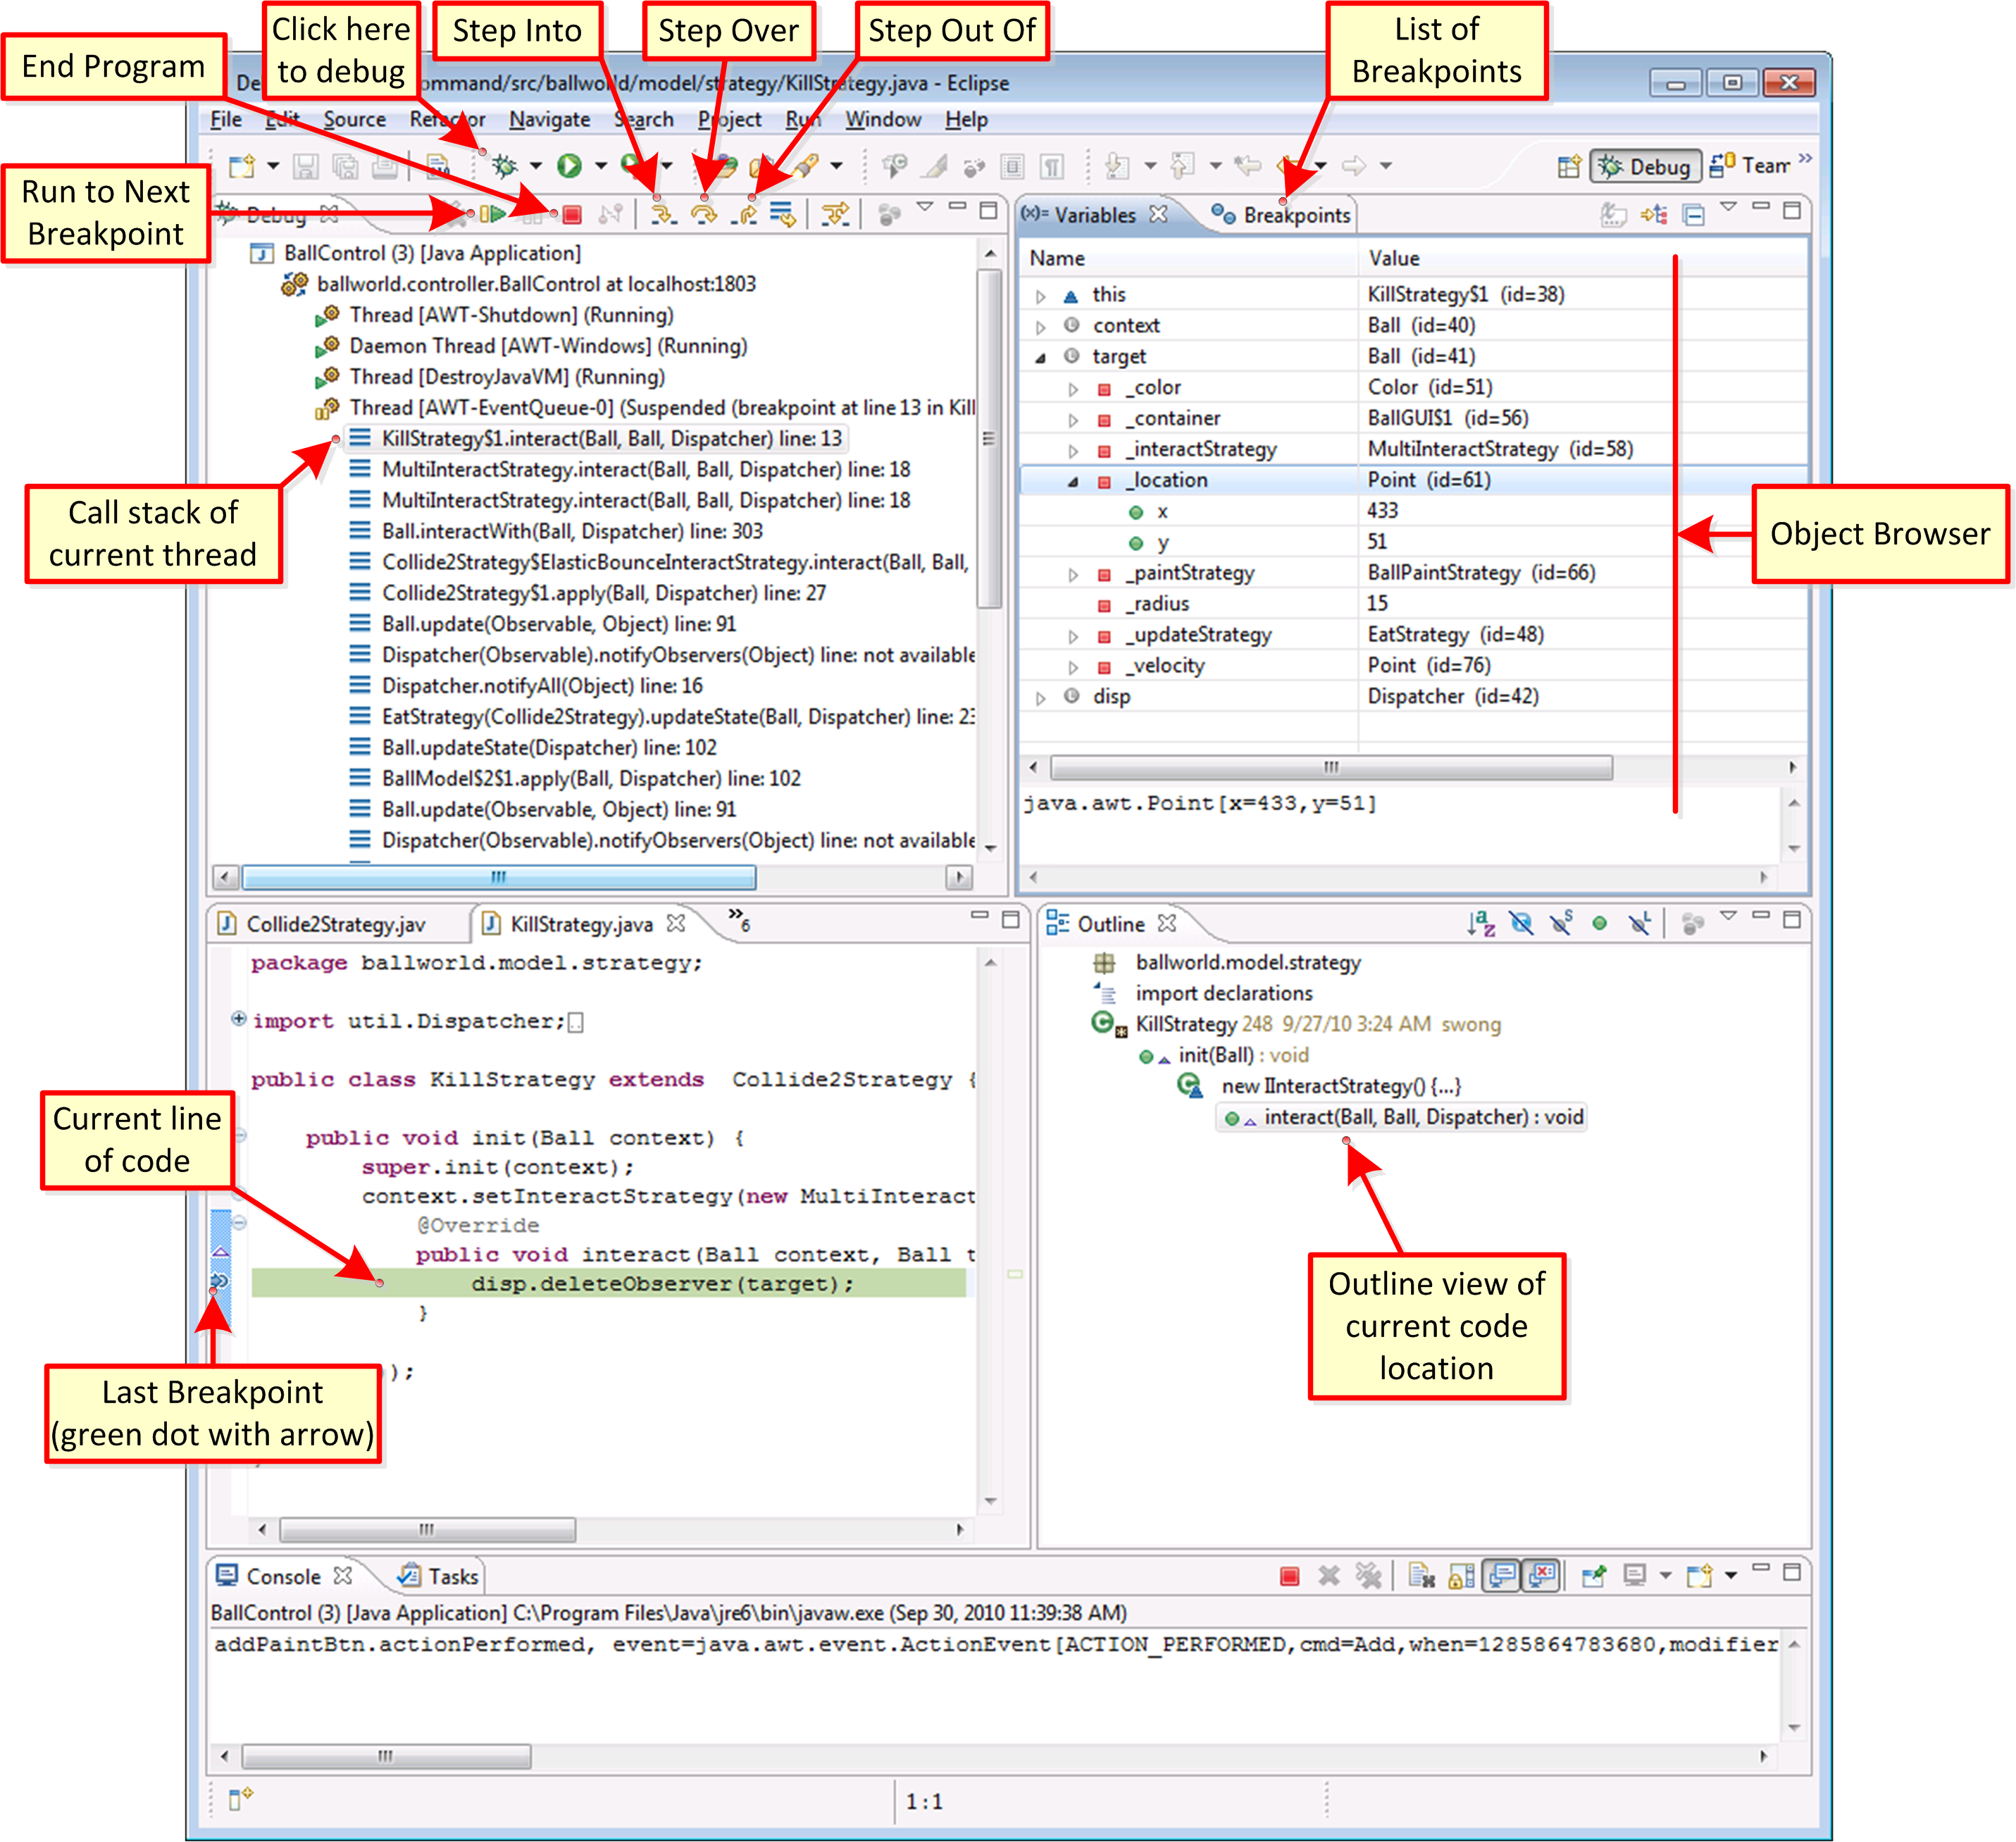
\includegraphics[width=0.7\columnwidth]{debug} 
    \bigskip
    \caption{IDE Eclipse - Debug}
\end{figure}
\bigskip
\bigskip
\section{Processo di Validazione}
Il processo di validazione è stato eseguito insieme al tutor di tirocionio \textit{Roberto Martina}. Durante gli ultimi giorni sono stati eseguiti tutti i test e confermata la validità della webapp prodotta rispetto al requisiti definiti all'inizio dello stage. \\
Oltre alla conformità ai requisiti è ritenuto parte fondamentale di validità del prodotto anche il rispetto dei canoni della struttura aziendale presente. \\
Il tutor ha posto quindi molta attenzione anche su questo aspetto dato che non seguire la struttura designata porta ad un uso errato dei \textit{pattern} e dei \textit{framework} utilizzati. La struttura del codice aziendale è costruita con la consapevolezza di agevolare il programmatore nella creazione di nuove classi.